\documentclass{article}

\usepackage{graphicx}
\usepackage{tikz}
\usepackage{tikzsymbols}
\usetikzlibrary{calc,patterns,shapes.geometric}
\pagestyle{empty}
\usepackage[margin=0pt]{geometry}
\geometry{papersize={14in,12in}}

\def\centerarc[#1](#2)(#3:#4:#5){\draw[#1] ($(#2)+({#5*cos(#3)},{#5*sin(#3)})$) arc (#3:#4:#5);}

\begin{document}
	\begin{figure}
		\centering
		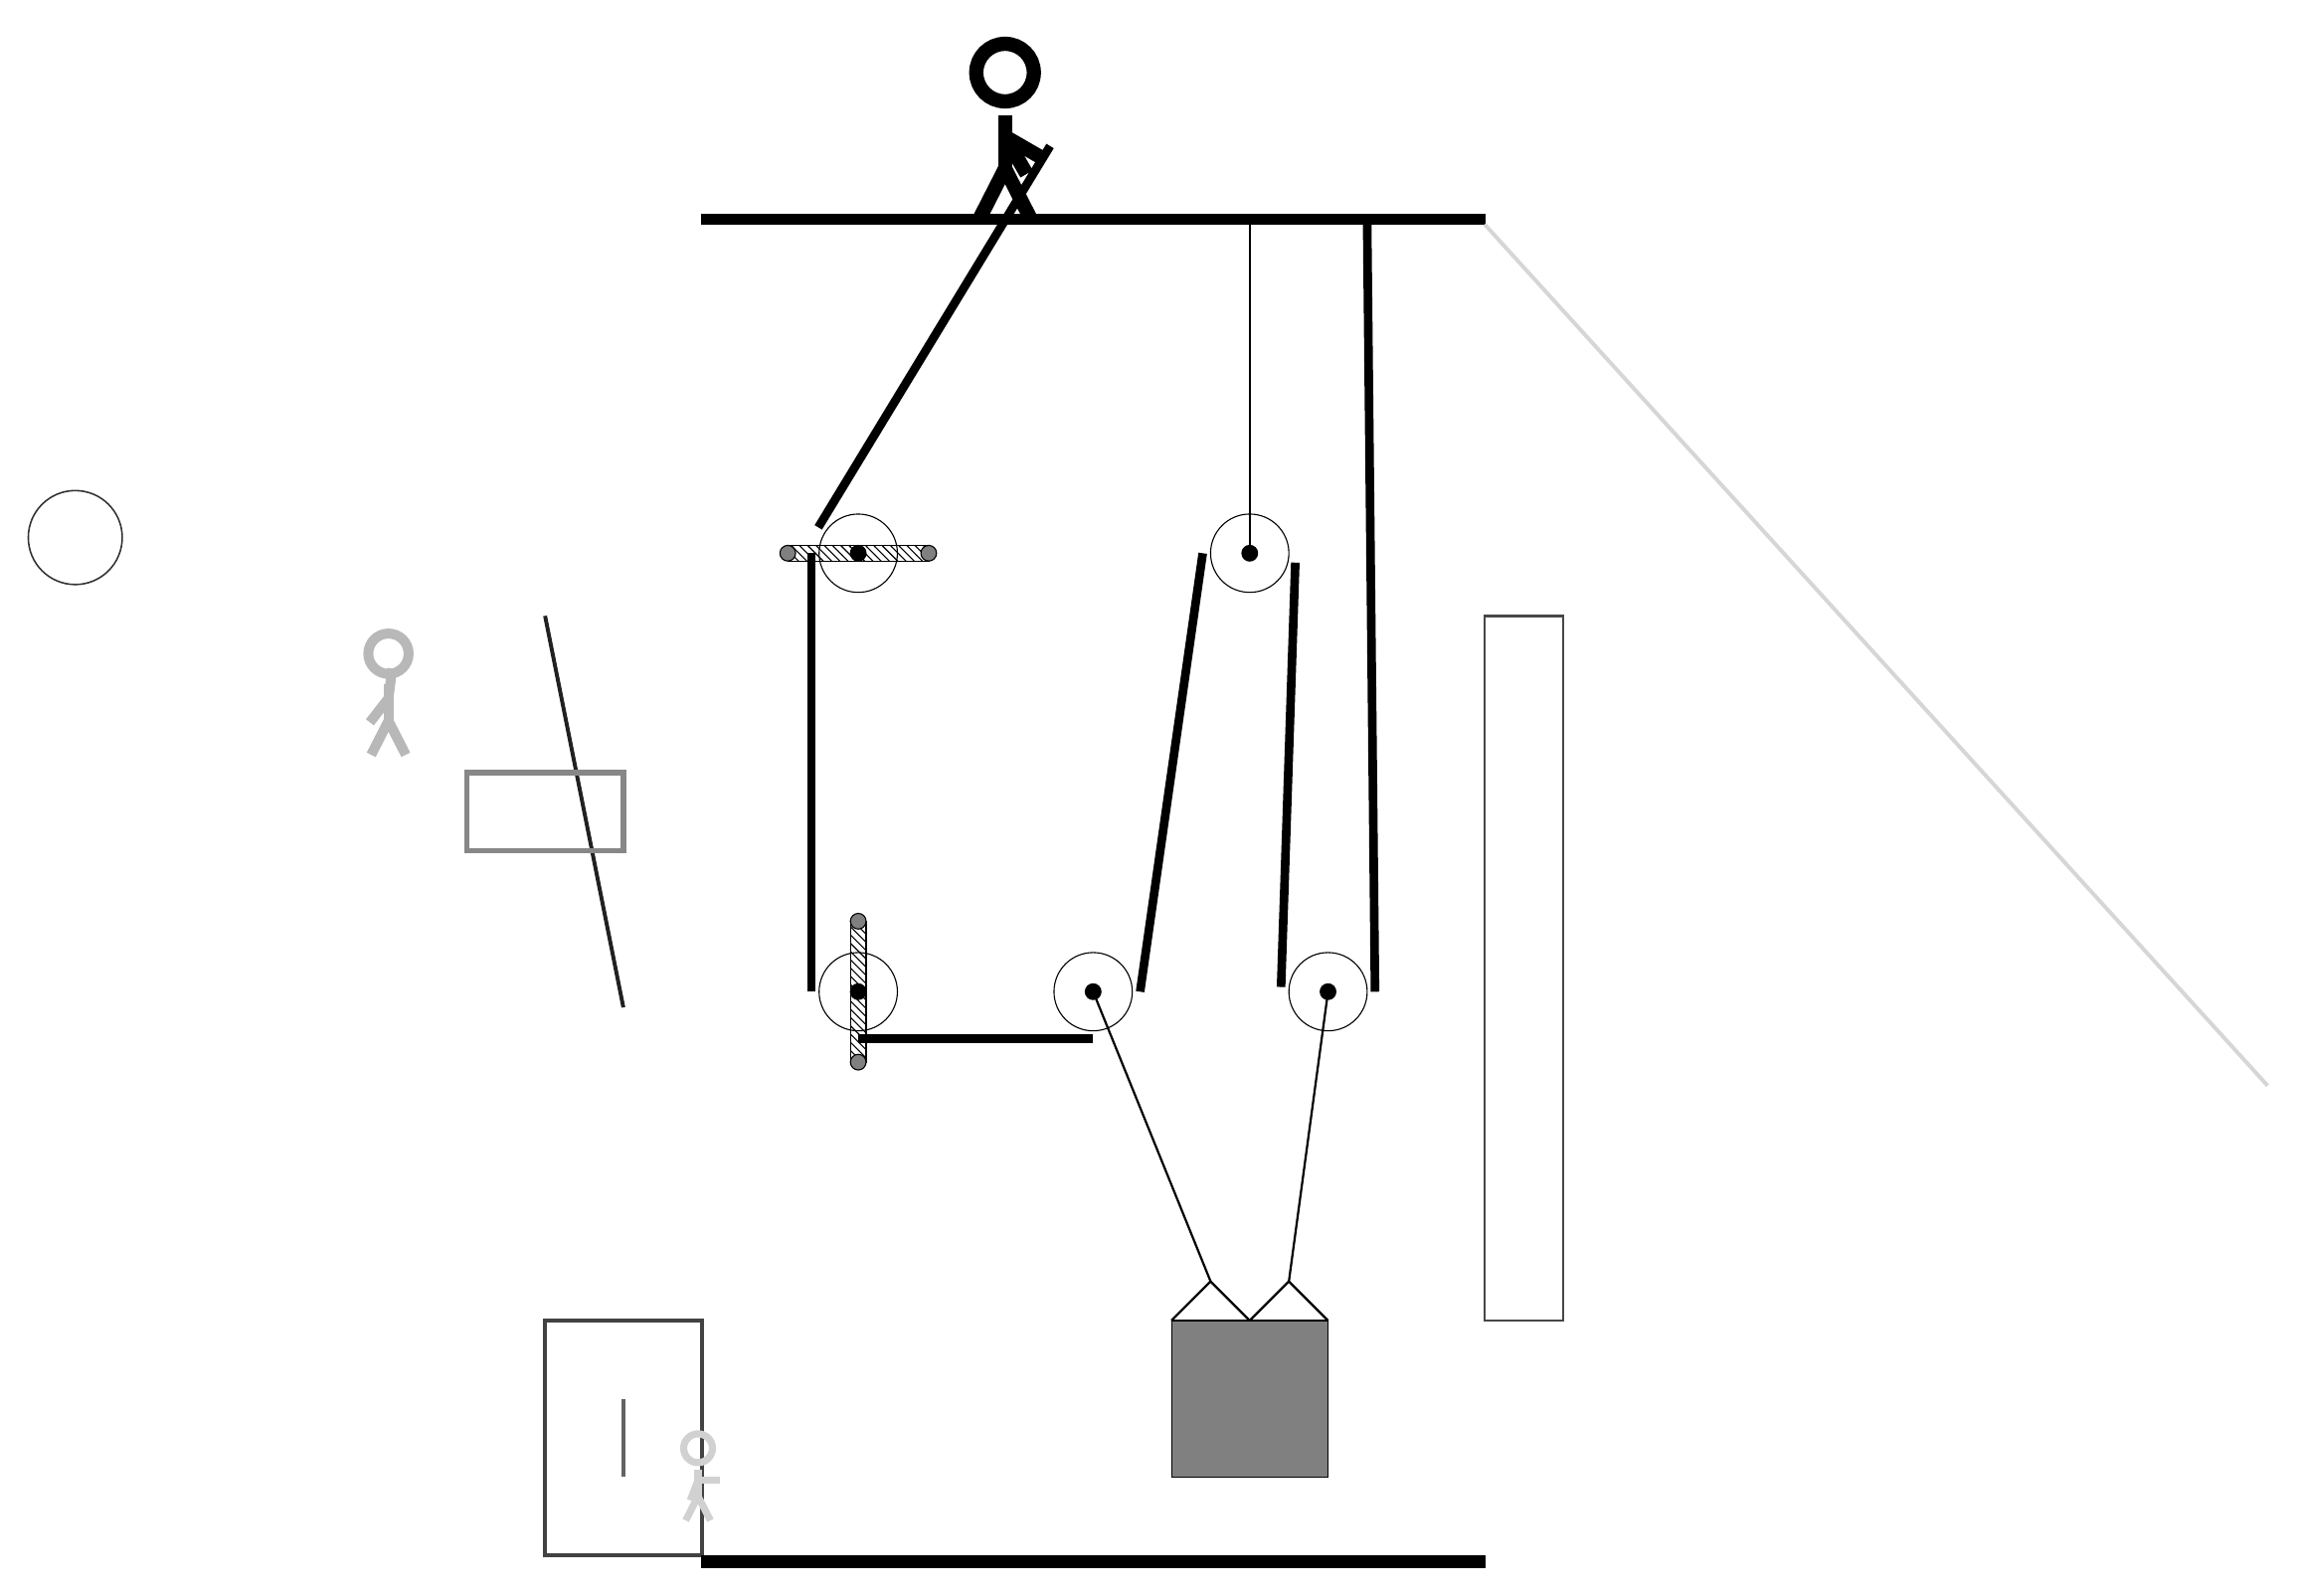
\begin{tikzpicture}
			%%%%% START %%%%%
			
			\draw[fill=black] (-4, 14) rectangle (6, 14.125);
			
			\draw (1, 4.2) circle (0.5);
			\draw[fill=black] (1, 4.2) circle (0.1);
			
			\draw (3, 9.8) circle (0.5);
			\draw[fill=black] (3, 9.8) circle (0.1);
			\draw[thick] (3, 9.8) -- (3, 14);
			
			\draw (4, 4.2) circle (0.5);
			\draw[fill=black] (4, 4.2) circle (0.1);
			
			\draw[thick] (4, 4.2) -- (3.5, 0.5);
			\draw[thick] (1, 4.2) -- (2.5, 0.5);
			\draw[thick]  (2, 0) -- (2.5, 0.5) -- (3, 0);
			\draw[thick]  (3, 0) -- (3.5, 0.5) -- (4, 0);
			\draw[fill=black!50] (2, 0) rectangle (4, -2);
			
			\draw[line width=0.3mm, color=black!72] (6, 9) rectangle (7, 0);
			
			\draw[line width=0.5mm, color=black!61](-5, -1) -- (-5, -2);
			\draw[line width=0.5mm, color=black!74] (-6, 0) rectangle (-4, -3);
			\draw[line width=0.5mm, color=black!87](-6, 9) -- (-5, 4);
			\node[line width=0.2mm, color=black!18] at (-4, -2) {\Strichmaxerl[5][69][0]};
			\draw[line width=0.5mm, color=black!16](6, 14) -- (16, 3);
			\node[line width=0.2mm, color=black!28] at (-8, 8) {\Strichmaxerl[7][52][83]};
			
			\draw[line width=0.7mm, color=black!47] (-5, 7) rectangle (-7, 6);
			\draw [line width=0.2mm, color=black!80](-12, 10) circle (0.6);
			
			
			\draw (-2, 4.2) circle (0.5);
			\draw[fill=black] (-2, 4.2) circle (0.1);
			\draw[pattern=north west lines, pattern color=black] (-2.1, 5.1) rectangle (-1.9, 3.3);
			\draw[fill=black!50] (-2, 5.1) circle (0.1);
			\draw[fill=black!50] (-2, 3.3) circle (0.1);
			
			\draw (-2, 9.8) circle (0.5);
			\draw[fill=black] (-2, 9.8) circle (0.1);
			\draw[pattern=north west lines, pattern color=black] (-2.9, 9.9) rectangle (-1.1, 9.7);
			\draw[fill=black!50] (-2.9, 9.8) circle (0.1);
			\draw[fill=black!50] (-1.1, 9.8) circle (0.1);
			
			\draw[line width=1.1mm] (0.45, 15) -- (-2.51, 10.13);
			\centerarc[line width=1.1mm](-2, 9.8)(135:180:0.6);
			\draw[line width=1.1mm] (-2.6, 9.8) -- (-2.6, 4.2);
			\centerarc[line width=1.1mm](-2, 4.2)(180:270:0.6);
			\draw[line width=1.1mm](-2, 3.6) -- (1, 3.6);
			\centerarc[line width=1.1mm](1, 4.2)(270:360:0.6);
			\draw[line width=1.1mm] (1.6, 4.2) -- (2.4, 9.8);
			\centerarc[line width=1.1mm](3, 9.8)(-20:180:0.6);
			\draw[line width=1.1mm](3.582, 9.68) -- (3.4, 4.26);
			\centerarc[line width=1.1mm](4, 4.2)(160:360:0.6);
			\draw[line width=1.1mm](4.6, 4.2) -- (4.5, 14);
			
			\node at (-0.07, 15.2) {\Strichmaxerl[10][120][-30]};
			
			\draw[fill=black] (-4, -3) rectangle (6, -3.15);
			
			%%%%% END %%%%%
		\end{tikzpicture}
	\end{figure}	
\end{document}